\subsection{Client Side}\label{client side}

This chapter will introduce the design and architecture of the client side of our system. Section \ref{client introduction} will introduce the different components that make up the entire client, and includes a description of the different components that make up the client library. Next, section \ref{client use cases} will describe the use cases, and section \ref{textual client data flow} will take care of the data flow, followed by a detailed architecture description \ref{client architecture}. Finally, section \ref{client sequence diagrams} will go through the sequence diagrams.
		
    \subsubsection{Introduction}\label{client introduction}
The client architecture consists of the following components: The client application, the client library and the \gls{ms}.\footnote{Monitoring Service, a service that provides bandwidth monitoring, running on the same server as the Tactical Router} Additionally, the library makes use of some external components to do some of its work.
\\\\
\textbf{Component description:}
\\\\
Client application:\\
	The user-controlled applications that utilize web services. These must be modified to send all communication through the client library in order to get the prioritization it should have.
\\\\
Client library:\\
This component will handle all communication with the service providers, as well as authenticating users and prioritizing their messages, based on who they are, and what their current role is. The authorization will involve a component from the server side of the project, the identity server, which returns a token if the client is authorized. Client applications connect through a simple interface to provide credentials and data.
\\\\
Monitoring service (MS):\\
An external service, most likely residing on a tactical router(TR), that exposes the bandwidth of the active links on the TR it resides on. this information can be used by the library to help decide  if there is enough free capacity on the link to send more data, or if something must be done in order to maintain more connections over that link.
For our implementation we will most likely make extensive simplifying assumptions about this service since this is still in the research and development stage and therefore a proper implementation of it is unavailable. 
\\\\
\textbf{External libraries:}
\\\\
OpenSAML:\\
This component will be used to parse and manipulate \gls{xml}\footnote{\gls{xml} - eXtensible Markup Language} data in the form of SOAP and SAML. These are fairly extensive and complex data structures so a easy to use external library is essential here.
\\\\
Apache \gls{httpcomponents}:\\
A lightweight component for easily setting up and using HTTP connections.
While not strictly necessary this component will allow us to connect and communicate across networks far more easily than built in java components.

	\subsubsection{Use Cases}\label{client use cases}
		\textbf{Title:} Accept client info \\
		\textbf{Actors:} Client software, Client Library Interface \\
		\textbf{Main:}
		\begin{enumerate}
			\item Client software connects to the library interface
			\item Client delivers its credentials
			\item Credentials are passed from interface to sequencer.
			\item Credentials are sanity checked by sanity checker and passes.
			\item Credentials are passed from sequencer to Token manger, then to credential storage.
			\item Credentials are stored
			\item Buffer for previous tokens is flushed
		\end{enumerate}
		\textbf{Extension:} 
		\begin{itemize}
			  \item[] 4a. Credentials are obviously invalid
			  \item[] 5a. Return error
		\end{itemize}
		\\\\
		\textbf{Title:} Accept data to be sent \\
		\textbf{Actors:} Client software, Client Library Interface \\
		\textbf{Main:}
		\begin{enumerate}
			\item Client delivers data it wishes to send
			\item Data is passed to the sequencer.
			\item Sequencer creates DataObject
		\end{enumerate}
		\textbf{Extension:}
		\begin{itemize}
			 \item[] none
		\end{itemize}
		\textbf{Precondition:} Client has established connection to the Library interface and delivered its credentials. \\
		\textbf{See:} accept client info
		\\\\
		\textbf{Title:} Fetch Bandwidth info \\
		\textbf{Actors:} client library, Monitoring Service(MS) (probably on tactical router(TR)) \\
		\textbf{Main:}
		\begin{enumerate}
			\item Establish connection to MS
			\item Read MS’s bandwidth info for the route between it and the server.
			\item Set bandwidth info for this connection in the DataObject.
		\end{enumerate}
		\textbf{Extension:}
		\begin{itemize}
			  \item[] 3a. Bandwidth info not in MS
			  \item[] 4a. Connection is local, set bandwidth info to a default for local network.
		\end{itemize}
		\textbf{Precondition:} Client has delivered library both credentials and data to be sent (with a destination). \\
		\textbf{See:} Accept client credentials and Accept data to be sent 
		\\\\
		\textbf{Title:} Connect to server \\
		\textbf{Actors:} Client Library, Server \\
		\textbf{Main:}
		\begin{enumerate}	
			\item Connection manager connects to the server
			\item Set priority on socket based on SAML-token and related metadata
		\end{enumerate}
		\textbf{Extension:}
		\begin{itemize}
			  \item[] 1a. Unable to connect to server
			  \item[] 2a. Return error
		\end{itemize}
		\textbf{Precondition:} DataObject has been created, and contains both bandwidth info and a token \\
		\textbf{See:} Accept client credentials, Accept data to be sent and Fetch bandwidth info
		\\\\
		\textbf{Title:} Get SAML token \\
		\textbf{Actors:} Client library, Server \\
		\textbf{Main:}
		\begin{enumerate}
			\item Client library sends client credentials to server
			\item Server verifies the credentials
			\item Server returns SAML-token
			\item Token is parsed into Token object
			\item Token object is put into DataObject.
		\end{enumerate}
		\textbf{Extension:}
		\begin{itemize}
			  \item 2a. Client credentials not valid
			  \item 3a. Server returns error
			  \item 4a. Client library throws error
		\end{itemize}
		\textbf{Precondition:} Client has given library credentials and data to send, and a SAML token for the destination doesn’t already exist. Connection to server established. \\
		\textbf{See:} Accept client credentials, Accept data to be sent, Fetch bandwidth info and Connect to server
		\\\\
		\textbf{Title:} Transaction towards server \\
		\textbf{Actors:} Client lib, server, client \\
		\textbf{Main:}
		\begin{enumerate}
			\item MessageHandler sends buffered data to server
			\item Server returns reply to data.
			\item The ReturnObject in the DataObject gets the data from the server.
			\item MessageHandler send data to sequencer.
			\item Sequencer sends data to interface (QosClient)
			\item Client fires a data received event to all listeners.
		\end{enumerate}
		\textbf{Extension:}
		\begin{itemize}
			 \item[] 2a. Server unavailable, reply doesn’t arrive within timeout, etc.
			 \item[] 3a. Throw error.
		\end{itemize}
		\textbf{Precondition:} Data to send exists, SAML token is in cache, connection to server active.\\
		\textbf{See:} Accept client credentials, Accept data to be sent, Fetch bandwidth info, Connect to server and Get SAML token
		
		
	\subsubsection{Data Flow}\label{textual client data flow}
        
    \begin{figure}[h]
        \centering
        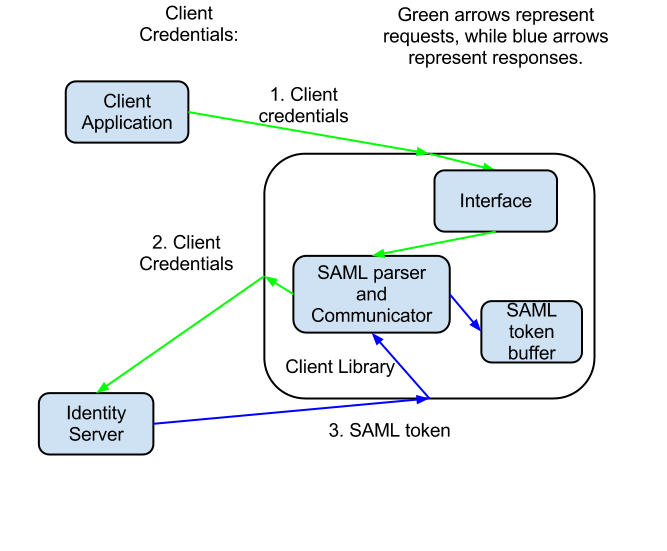
\includegraphics[scale=0.5]{ClientCredentialsDataFlowDiagram}
        \caption{Client Data Flow}
        \label{fig:ClientCredentialsDataFlowDiagram}
    \end{figure}
    
    \begin{figure}[h]
        \centering
        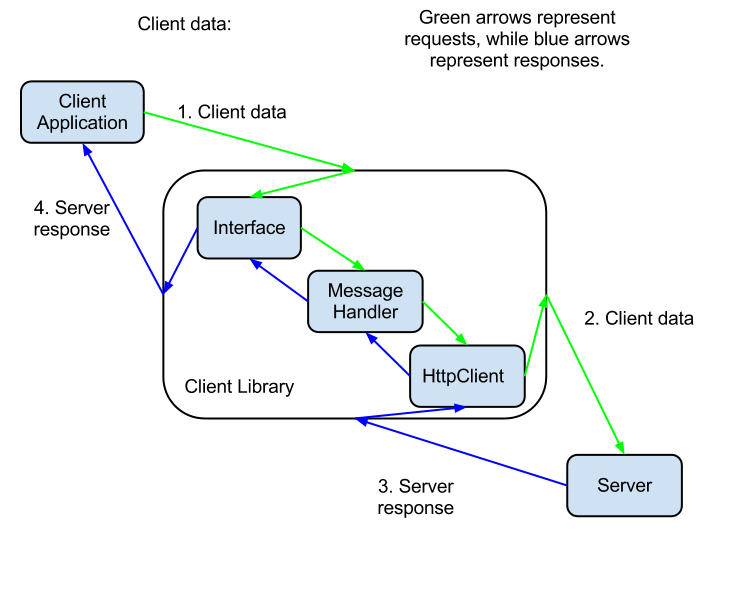
\includegraphics[scale=0.5]{ClientDataFlowDiagram}
        \caption{Client Credentials Flow}
        \label{fig:ClientDataFlowDiagram}
    \end{figure}
    
		Client credentials
		\begin{enumerate}
			\item From client application
			\item To client library via API/interface
			\item Via SAML to ID-server
			\item Back to client library as valid SAML-token
			\item Stored in library until client App changes credentials
		\end{enumerate}
		\\\\
		Bandwidth/link data
		\begin{enumerate}
			\item Generated by the Monitoring Service
			\item Delivered to clients and servers on request
		\end{enumerate}
		\\\\
		Client data
		\begin{enumerate}
			\item Generated by client application
			\item Sent to client library via API/interface
			\item Buffered in library
			\item Sent from library to server
			\item Answer returned to client through library
		\end{enumerate}
		
	\subsubsection{Architecture}\label{client architecture}
		\begin{figure}[h]
			\centering	
			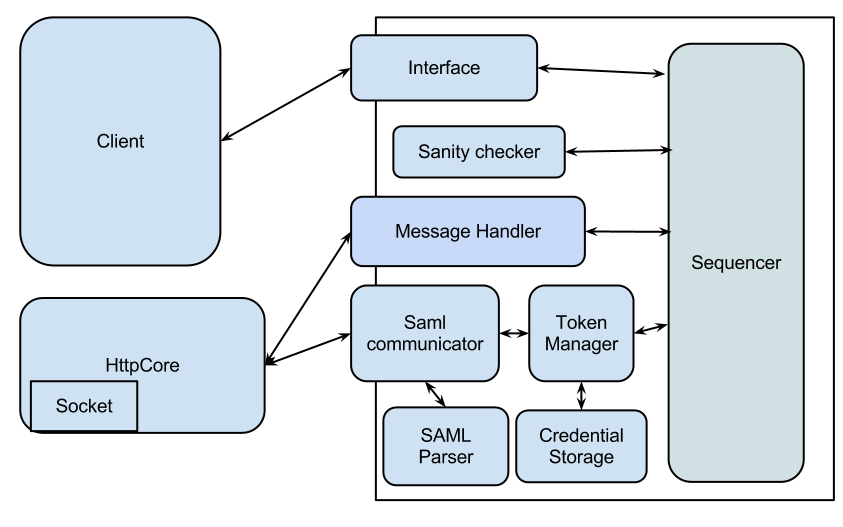
\includegraphics[width=\textwidth]{Detailedclientarchitecture}
			\caption{Detailed Client Architecture}
			\label{fig:DetailedClientArchitecture}
		\end{figure}

		\textbf{Interface} \\
Known in the class diagram as “QosClient”, responsible for providing a clean and easy to use interface for the clients.
\\\\
		\textbf{Sequencer} \\
The central piece of the client library. Responsible for keeping a record of all other modules in the system and communicate between them as well as making sure everything happens in the right order.
\\\\
		\textbf{Sanity checker} \\
This module is simply there to do some easy verification of data that comes from the client, to make sure that it isn’t faulty in any obvious way. (e.g: Data that isn’t xml, or credentials that are empty)
\\\\
		\textbf{Token Manager} \\
This provides a nice and clean interface for the sequencer to store credentials and fetch tokens for data transmissions.
\\\\
		\textbf{Saml Communicator} \\
This module will take care of the communication between the client library and the identity server.
\\\\
		\textbf{Saml Parser} \\
This takes the reply from the identity server and parses it into a token object so that it can be easily used and stored.
\\\\
		\textbf{Credential Storage} \\
Responsible for storing token objects as well as user supplied credentials. Also makes sure that no token objects are returned if they are invalid or expired.
\\\\
		\textbf{MsCommunicator} \\
Responsible for communicating with the monitoring service to get information about the bandwidth available to a given destination, as well as supplying some identifying information for the route used.

	\subsubsection{Sequence Diagrams}\label{client sequence diagrams}
		\begin{figure}[H]
			\centering	
			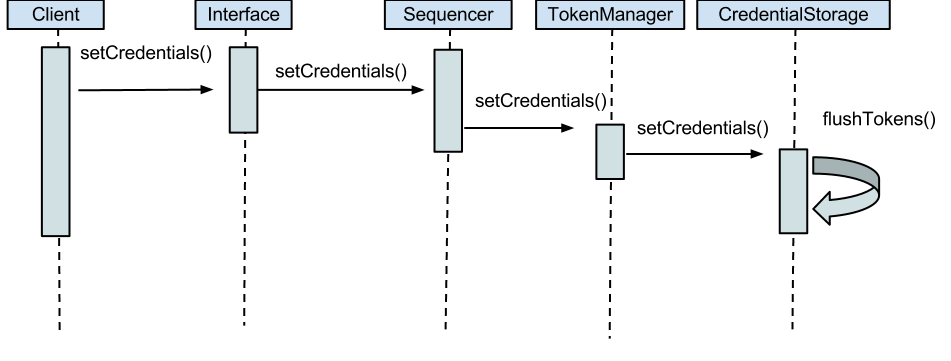
\includegraphics[width=\textwidth]{CliSeqDiaAcceptclientinfo}
			\caption{Accept client info}
			\label{fig:CliSeqDiaAcceptclientinfo}
		\end{figure}
		\begin{figure}[H]
			\centering	
			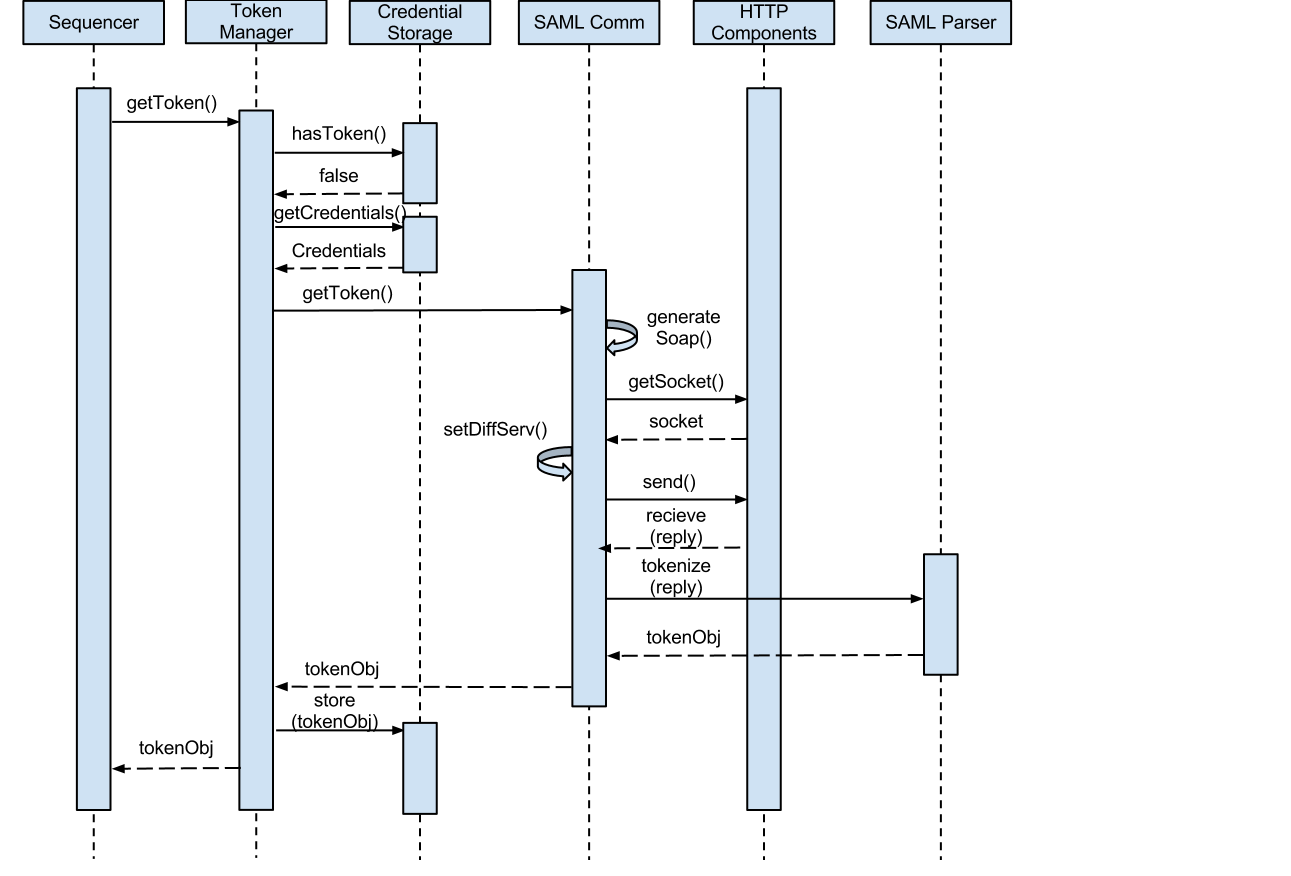
\includegraphics[scale=0.4, angle=-90]{CliSeqDiaGettingnon-storedtoken}
			\caption{Getting non-stored token}
			\label{fig:CliSeqDiaGettingnon-storedtoken}
		\end{figure}
		\begin{figure}[H]
			\centering	
			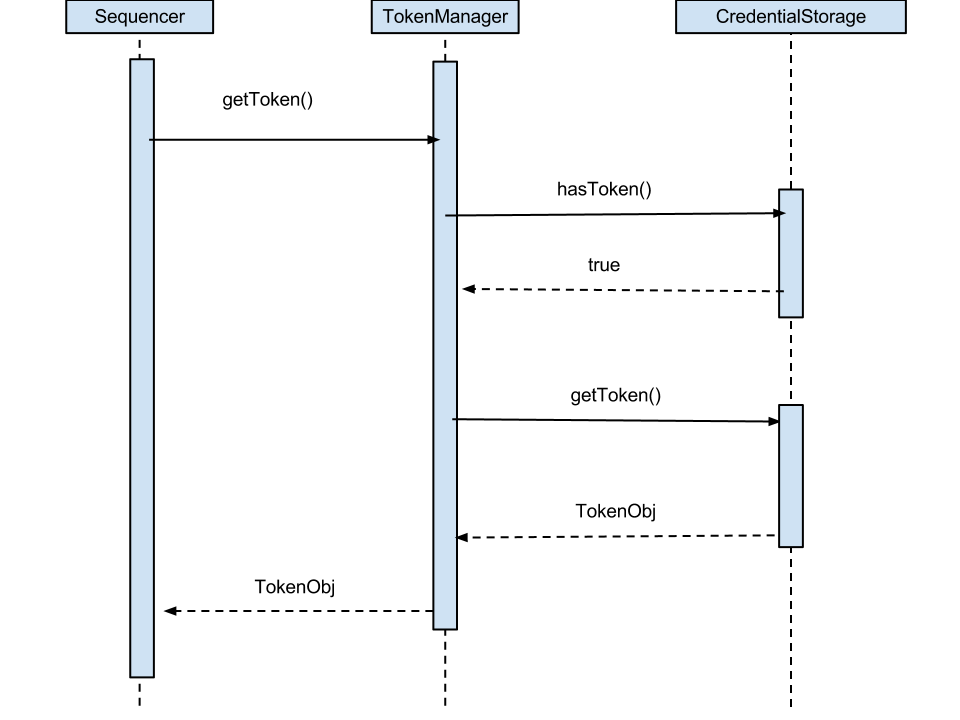
\includegraphics[scale=0.4, angle=-90]{CliSeqDiaGettingStoredToken}
			\caption{Getting stored token}
			\label{fig:CliSeqDiaGettingStoredToken}
		\end{figure}
		\begin{figure}[H]
			\centering	
			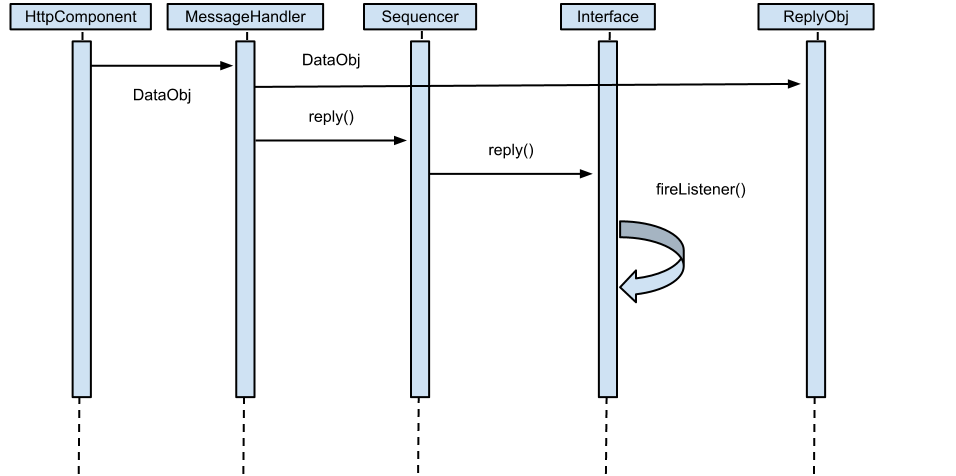
\includegraphics[scale=0.4, angle=-90]{CliSeqDiaReceivereply}
			\caption{Receive reply}
			\label{fig:CliSeqDiaReceivereply}
		\end{figure}
		\begin{figure}[H]
			\centering	
			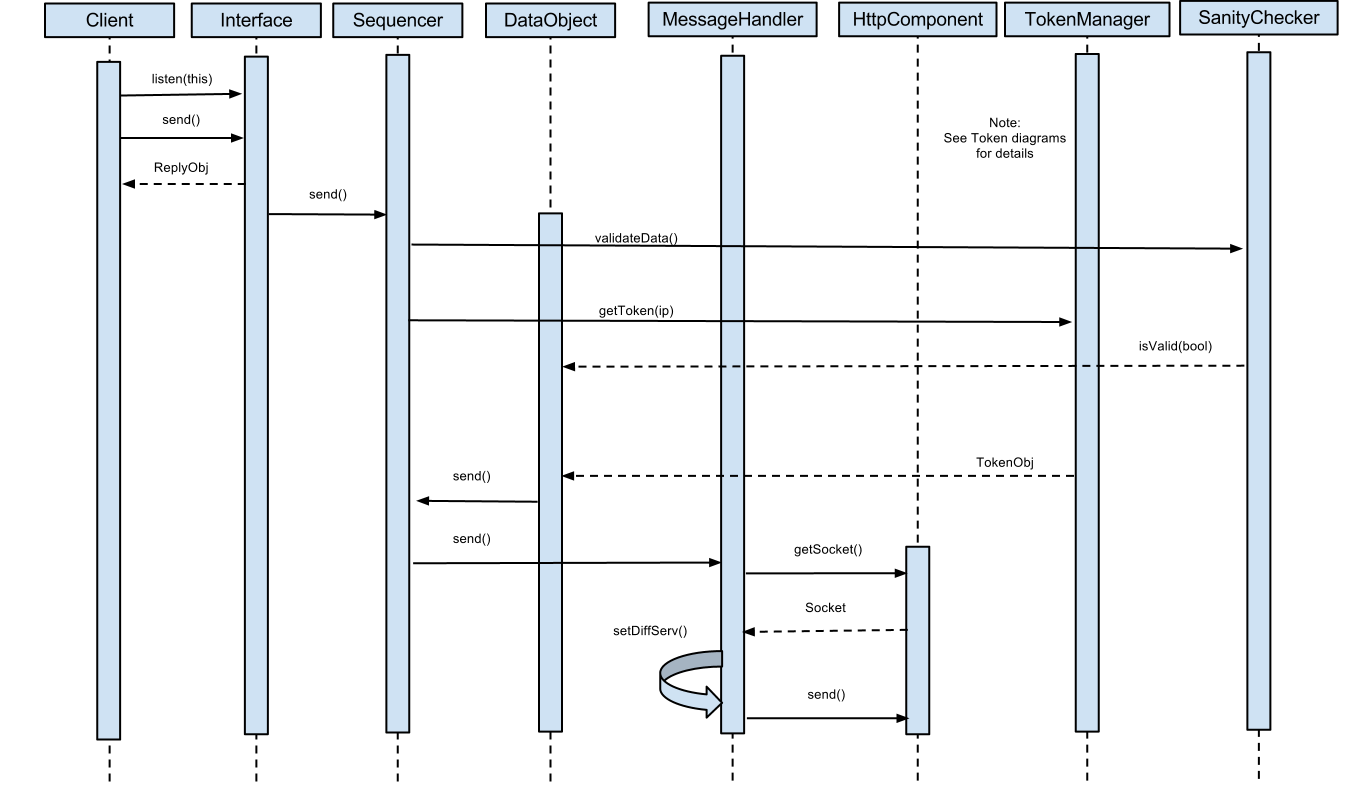
\includegraphics[scale=0.4, angle=-90]{CliSeqDiaSendData}
			\caption{Send data}
			\label{fig:CliSeqDiaSendData}
		\end{figure}

		

